\chapter{Theoretical Background}
\label{chap:background}

This chapter provides the theory essential to understand the major components of the thesis. Prior knowledge of Artificial Neural Networks \cite{theory_ann_wiki} and fundamental concepts of Deep Learning \cite{theory_dl} is assumed.

\section{Preliminary Concepts}
\label{sec:Preliminary}

\subsection{Autoencoder}
Autoencoders are a variant of \acp{ann}, which are designed to learn an identity function that generates the input data sample back. The network has a bottleneck($z$), dividing the network into two parts, an encoder and a decoder as illustrated in Fig \ref{fig:ae_arch}. The first network learns to compress the high dimensional input data to a low dimensional intermediate representation, \textit{latent representation}, at the bottleneck. While the second network learns to reconstruct the data from the latent distribution. Thus learning to efficiently compress the data.

\begin{figure}[h]
    \centering
    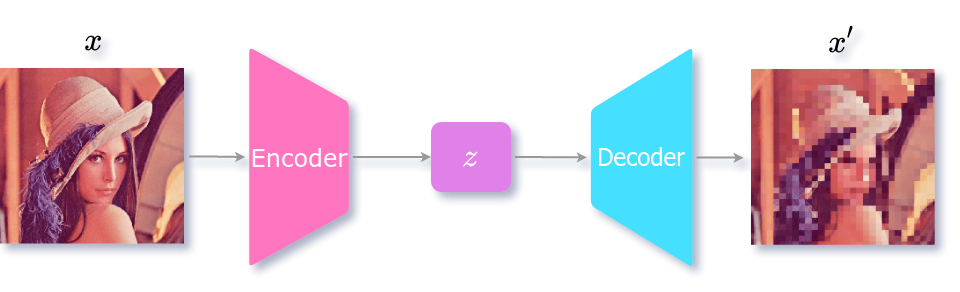
\includegraphics[scale=0.2]{figures/arch/ae_arch.png}
    \caption{Illustration of autoencoder architecture. Image source \cite{deepimageprior}}
    \label{fig:ae_arch}
\end{figure}

To put it in other words, in the process of learning to reconstruct the data, the encoder learns to filter the most important features of the given data distribution, so as it preserves the complete properties within the limits of the bottleneck. While the decoder learns comparatively general properties of the distribution which are used along with the compact latent representation from the encoder to fully recover the data distribution. The network is trained to minimize the similarity between the reconstruction and the original data sample. This similarity can be determined by metrics such as \ac{mse}, \ac{l1} or Cross-Entropy loss.

The idea of an autoencoder dates back to the '80s proposed as a method for pre-training and feature learning \cite{ballard1987modular, rumelhart1985learning}, learned dimensionality reduction \cite{hinton_dimentionality}. In recent years, autoencoders are most popularly used as generative networks leveraging their ability to learn feature representations in an unsupervised way. Another interesting variant of autoencoders is the denoising autoencoder \cite{vincent2008extracting}, where the input is a noised data and the decoder generates original data without noise. This variant is further evolved to accomplish the tasks of image denoising, watermark removal, inpainting, super-resolution, colorization, de-colorization, and compression \cite{zhang2016colorful, imagedenoisingpaper,deepimageprior}. 

\subsection{Variational Autoencoders}
\label{subsec:vae}
\acp{vae}, unlike standard autoencoders, learn to encode a data sample $x$ as a probabilistic distribution rather than a deterministic value for the latent attribute \cite{jeremy_jordan_2018}. The encoder $q$ produces the probabilistic distribution by predicting two vectors that represent the mean $\mu$ and standard deviation $\sigma$ of distribution for each of the latent attributes of $x$. And the decoder $p$ takes a random sample $z$ from this distribution to recover the sample as illustrated in Fig \ref{fig:vae_arch}.

\begin{figure}[h]
    \centering
    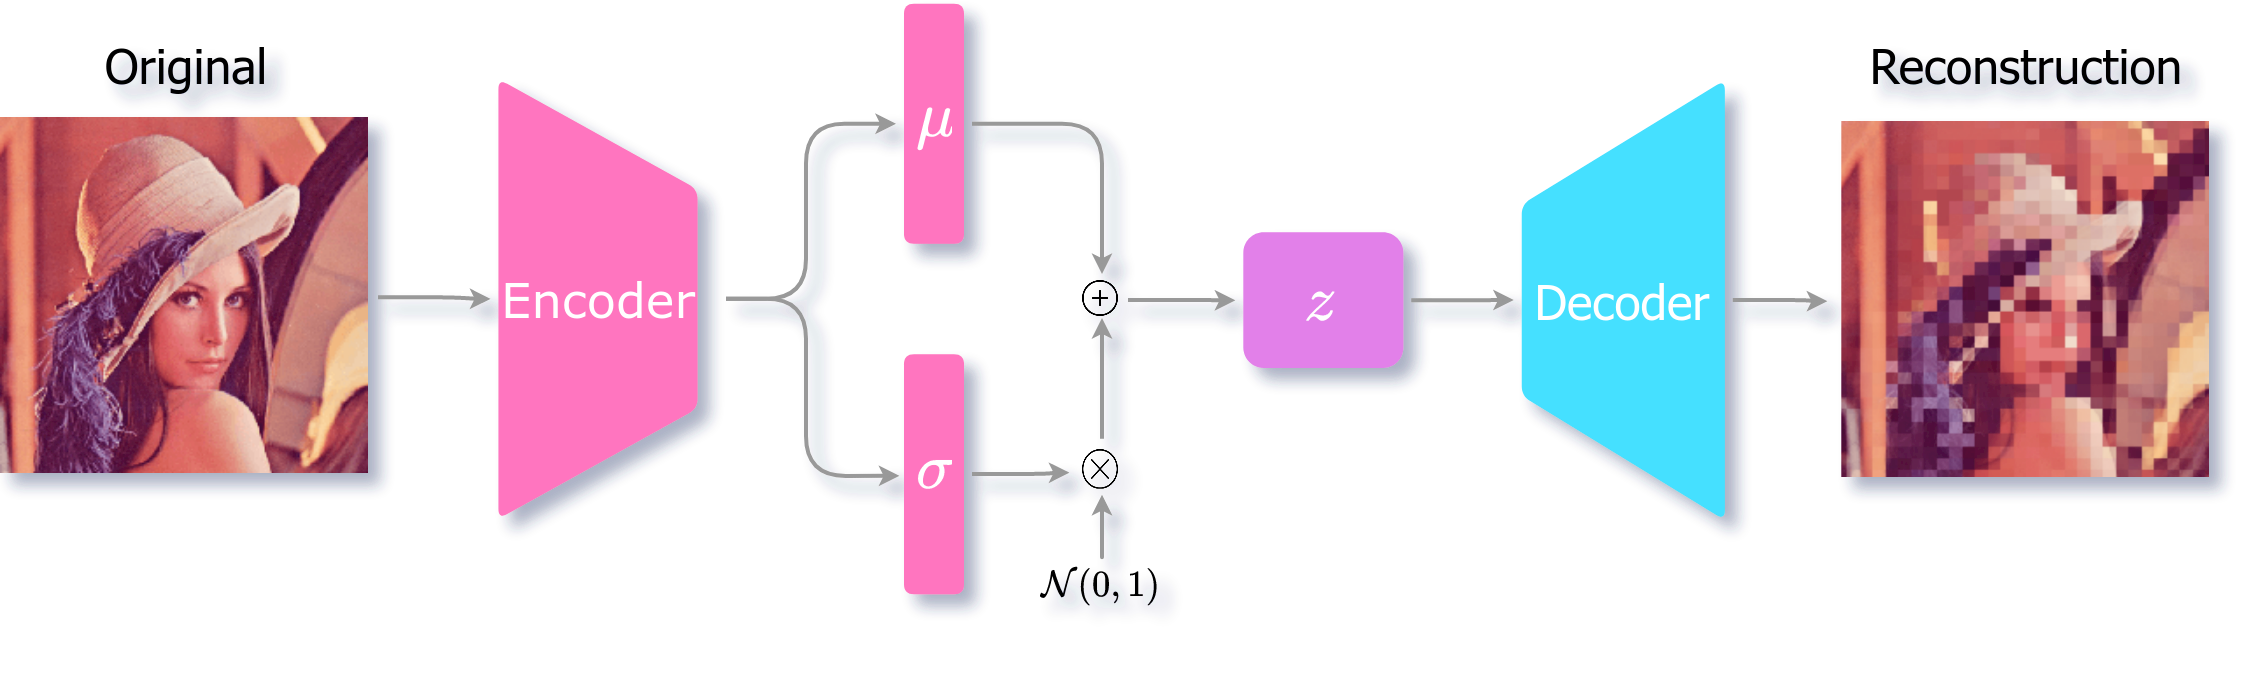
\includegraphics[scale=0.2]{figures/arch/vae_arch.png}
    \caption{Illustration of Variational Autoencoder architecture.}
    \label{fig:vae_arch}
\end{figure}

To put it formally, we have a hidden variable $z$ which generates $x$. Since we only have $x$ and would want to learn $z$ i.e $p(z | x)$. But computing this posterior distribution is hard as computing $p(x)$ Eqn. \ref{eqn:pofx} is usually intractable \cite{kingma2013autoencoding}.

\begin{equation}\label{eqn:pofx}
    \begin{gathered}[b]
        p(z | x)=\frac{p(x | z) p(z)}{p(x)} \\
        p(x)=\int p(x | z) p(z) dz
    \end{gathered}
\end{equation}

Hence, we try to approximate the posterior distribution by another distribution $q(z|x)$ (the encoder) using variational inference. Variational inference uses optimization to find a distribution that minimizes the \ac{kld} to the posterior distribution, $\min D_{\mathrm{KL}}(q(z| x) \| p(z| x))$ while trying to keep the learnt distribution close to the true prior distribution $p(z)$ \cite{variational_inference}. The prior $p(z)$ is usually assumed to be a unit gaussian distribution. The above can also be achieved by maximizing:

\begin{equation} \label{eqn:minKLd}
    \begin{gathered}[b]
        \max \mathbb{E}_{q(z | x)} \log p(x | z) - D_{\mathrm{KL}}(q(z | x) || p(z))
    \end{gathered}
\end{equation}

The first term in the above equation makes sure the reconstruction is close to the data sample $x$, while the second term tries to keep the learned distribution $q(z|x)$ close to the true prior $p(z)$. Hence the loss term to \textit{minimize} while training the \ac{vae} is $\mathcal{L}_{\mathrm{VAE}}$ Eqn. \ref{eqn:vae_loss}.

\begin{equation} \label{eqn:vae_loss}
    \begin{gathered}[b]
        \mathcal{L}_{\mathrm{VAE}}=-\mathbb{E}_{q(z | x)} \log p(x | z) + D_{\mathrm{KL}}(q(z | x) || p(z)) =\mathcal{L}_{\text {recon}} +\mathcal{L}_{\text {prior }}
    \end{gathered}
\end{equation}

However, the reconstruction error in the loss requires sampling $z$, which is a stochastic process and it is not possible to perform backpropagation. To address this problem, the \textbf{\textit{reparametrization trick}} is used. Where $\epsilon$ is randomly sampled from a unit gaussian distribution $\mathcal{N}(0,1)$ and is used to scale the standard deviation $\sigma$ of the latent distribution represented by the encoder $q_{\theta}(z|x)$. Where $\theta$ is the parameters of the encoder. The sum of the mean $\mu$ and the scaled standard deviation $\sigma \odot \epsilon$ gives $z$, which is now differentiable while being stochastic as illustrated in Fig \ref{fig:reparametrization_trick}.

\begin{figure}[h]
    \centering
    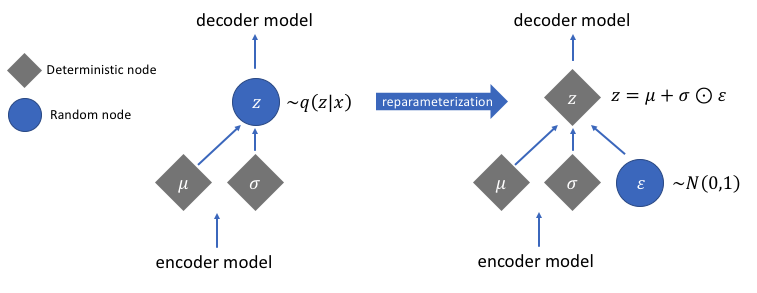
\includegraphics[scale=0.5]{figures/background/reparametrization_trick.png}
    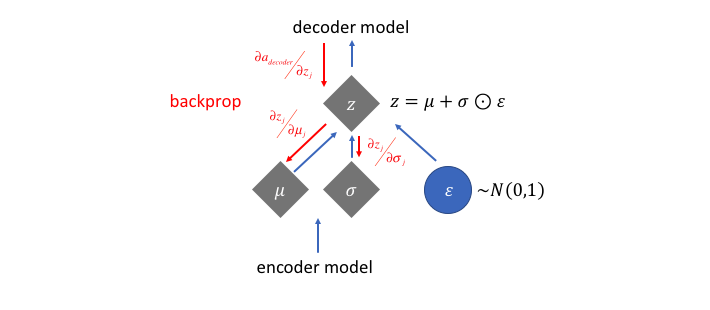
\includegraphics[scale=0.5]{figures/background/reparametrization_trick_backprop.png}
    \caption{Comparing the data flow with and without reparametrization trick followed by the backprop calculation. Image source \cite{jeremy_jordan_2018}}
    \label{fig:reparametrization_trick}
\end{figure}

Hence the learned latent space of a \ac{vae} is continuous, while that of a standard autoencoder is discrete and clustered. As the decoder of the \ac{vae} is trained to generate data from this continuous space, it can generate realistic data by randomly sampling from this infinitely large latent space as illustrated in the Fig \ref{fig:vae_latent_attribute}. This also enables smooth interpolation of data produced from one point in the latent space to another. In addition to that, we can also perform arithmetics in vector space, similar to the popular example from Natural Language Processing, $King - Man + Women = Queen$ but on much higher dimensional embedding space.

\begin{figure}[h]
    \centering
    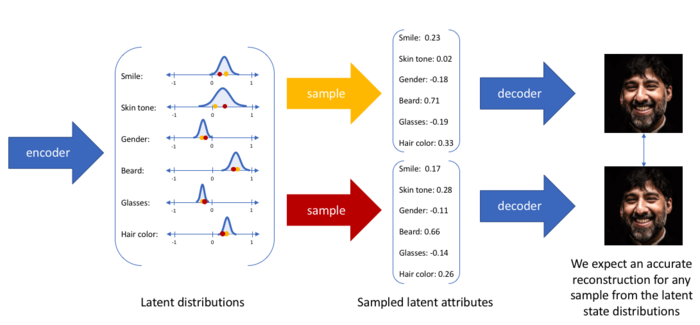
\includegraphics[scale=0.4]{figures/background/vae_latent_attribute.png}
    \caption{Probabilistic distribution of latent attributes. Image source \cite{jeremy_jordan_2018}}
    \label{fig:vae_latent_attribute}
\end{figure}

\subsection{Beta Variational Autoencoder}
\label{subsec:bvae}
A \ac{vae} without the \ac{kld} term is effectively a standard autoencoder. As discussed the \ac{kld} term encourages the network to learn a distribution rather than a single value. If the variance of the distribution is not high, then it is again similar to an autoencoder. The more enforcement from \ac{kld}, the diverse the distribution. The \ac{vae} is forced to disentangle the representations, i.e the lesser is the correlation between each dimension in the latent space. Such disentangled representations are very useful for generative models. More importantly, it improves the interpretability of the latent space and can be leveraged to generalize to different downstream tasks. This emphasis on the latent space distributions can be achieved by disentangled variational autoencoders or \ac{bvae}, where $\beta$ is the weight coefficient of the \ac{kld} term in the \ac{vae} loss function Eqn.\ref{eqn:vae_loss}. So, the loss for the \ac{bvae} is $\mathcal{L}_{\mathrm{VAE}}$ Eqn. \ref{eqn:bvae_loss}. The higher the beta the stronger the constrain on the disentanglement. However, this constraint will negatively affect the representation capability of the \ac{vae}.

\begin{equation} \label{eqn:bvae_loss}
    \begin{gathered}[b]
        \mathcal{L}_{\mathrm{VAE}}=-\mathbb{E}_{q(z | x)} \log p(x | z) + \beta (D_{\mathrm{KL}}(q(z | x) || p(z)))
    \end{gathered}
\end{equation}

\subsection{Generative Adversarial Networks}
\label{subsec:gan}
\ac{gan} is an \ac{ann} that is used for generative tasks, to make the prediction \textit{realistic}. A \ac{gan} is a combination of 2 networks namely, the generator $G$ and the discriminator $D$. The generator learns to map a random sample or say, noise $Z$ drawn from a latent distribution with density $p_{z}$ to a higher dimensional data distribution with density $p_{g}$. Whereas the discriminator takes the output of the generator and tries to differentiate real data samples $x$ from the fakes which do not belong to the real distribution $p_{r}$  as illustrated in Fig \ref{fig:gan_arch}.

\begin{figure}[h]
    \centering
    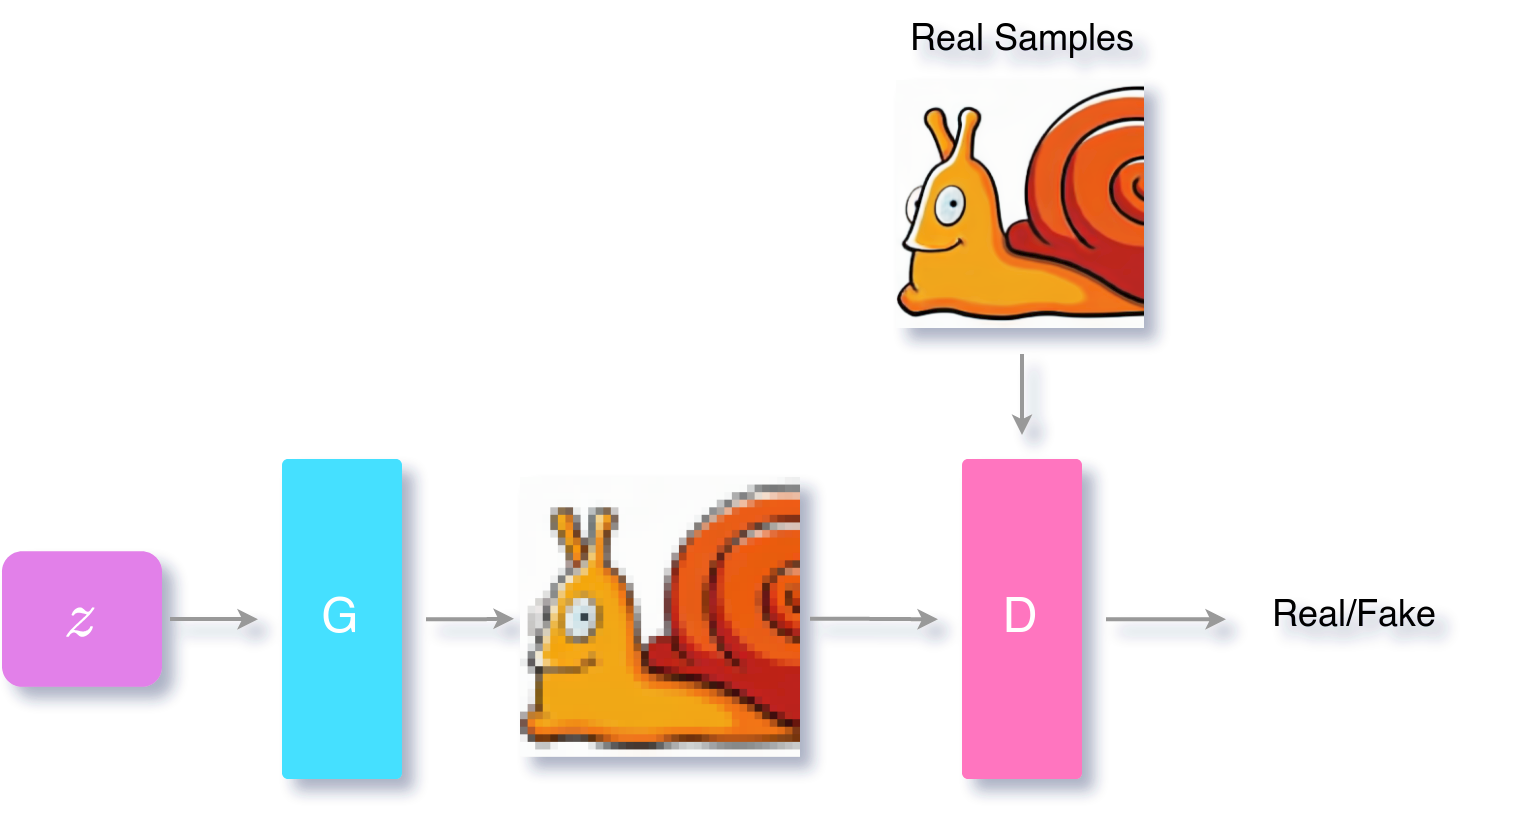
\includegraphics[scale=0.2]{figures/arch/gan_arch.png}
    \caption{Illustration of GAN architecture. G is the generator network and D is the discriminator network.}
    \label{fig:gan_arch}
\end{figure}

The goal of the generator is to produce samples, $G(z)$, that fool the discriminator into believing them as real samples. While the goal of the discriminator is to distinguish between the samples produced by the generator and the real samples by predicting reals as 1 and 0 for fakes. This inverse goal of the two networks can be viewed as a game of tug of war or a 2-player minimax game. The result of the game is that the generator would ideally learn to produce realistic data samples by sampling from prior $p_{g}(z)$. We effectively train $G$ to minimize $\log(1-D(G({z})))$ and $D$ to maximize $\log(D(x))$ making the loss function as $\mathcal{L}_{\mathrm{GAN}}$ Eqn. \ref{eqn:gan_loss}.

\begin{equation} \label{eqn:gan_loss}
    \begin{gathered}[b]
        {L}_{\mathrm{GAN}}=\mathbb{E}_{{x} \sim p_{r}(x)}[\log D({x})]+\mathbb{E}_{{z} \sim p_{z}(z)}[\log (1-D(G({z})))]
    \end{gathered}
\end{equation}

However, when it comes to training a \acp{gan}, practice is very different from theory. The training of the discriminator and generator is done iteratively and sequentially. But training the discriminator network to the optimal solution and then training the generator and repeating this loop is computationally challenging and would lead to overfitting the models on the finite dataset. To avoid this, the discriminator is trained for $k$ mini-batch iterations before training the generator for one iteration. This is to keep the discriminator close to optimality while slowly training the generator \cite{goodfellow2014generative}. The problem that arises here is that the generated samples are drastically different from the real samples as the generator has not yet learned to produce good samples. As the generator outputs samples close to noise, the discriminator easily distinguishes these samples from the real samples with high confidence. This saturates the loss term $\log (1-D(G(z)))$ very quick and leads to the problem of \textit{Vanishing Gradients}. Hence in practice, we train the generator $G$ to maximize $\log D(G(z))$ instead of minimizing $\log (1-D(G(z)))$, preventing the gradients from vanishing.

\begin{equation} \label{eqn:dg_of_x}
    \begin{aligned}[b]
        D_{G}^*(x) = & \frac{p_{r}(x)}{p_{r}(x)+p_{g}(x)} \\
        =            & \frac{1}{2}
    \end{aligned}
\end{equation}

At global optimality $p_{g}=p_{r}$, and for a given generator $G$, the discriminator at optimality is $D_{G}^*(x)$ Eqn. \ref{eqn:dg_of_x}. Hence the virtual cost $C(G)$ \cite{goodfellow2014generative} when $p_{g}=p_{r}$ is:

\begin{equation} \label{eqn:c_of_g}
    \begin{aligned}
        C(G) & = \max _{D} V(G, D)                                                                                                                                          \\
             & =\mathbb{E}_{x \sim p_{r}}\left[\log D_{G}^{*}(x)\right]+\mathbb{E}_{z \sim p_{z}}\left[\log \left(1-D_{G}^{*}(G(z))\right)\right]                           \\
             & =\mathbb{E}_{x \sim p_{r}}\left[\log D_{G}^{*}(x)\right]+\mathbb{E}_{x \sim p_{g}}\left[\log \left(1-D_{G}^{*}(x)\right)\right]                              \\
             & =\mathbb{E}_{x \sim p_{r}}\left[\log \frac{p_{r}(x)}{P_{r}(x)+p_{g}(x)}\right]+\mathbb{E}_{x \sim p_{g}}\left[\log \frac{p_{g}(x)}{p_{r}(x)+p_{g}(x)}\right] \\
             & =-\log (4)+ D_{\mathrm{KL}}\left(p_{r} \| \frac{p_{r}+p_{g}}{2}\right)+D_{\mathrm{KL}}\left(p_{g} \| \frac{p_{r}+p_{g}}{2}\right)                            \\
             & =-\log(4) + 2 \cdot  \mathrm{JSD}(p_{r} \| p_{g})
    \end{aligned}
\end{equation}

The \ac{jsd} between two distributions is always non-negative and will be equal to zero only when both the distributions are equal \cite{js_divergence}. As we derived in Eqn. \ref{eqn:c_of_g} above, the best value of $C$ i.e $-\log 4$ is possible only when $p_{g}=p_{r}$. It is hard to stabilize the \ac{gan}'s minimax game \cite{martin2017principled}. It requires carefully tuned hyperparameters to maintain an equilibrium between the two players. Failing to find the proper balance between the networks leads to the problem of \textit{Non-Convergence}, where the training oscillates and never converge. When the generator is not strong enough and learns to produce samples that fool the discriminator, it eventually would restrict itself to only learn to produce such samples. This problem is referred to as \textit{Mode Collapse} \cite{commonganprobs}. There are many hacks as well as principled approaches that are formulated to handle these problems with considerable success \cite{openaigan2wgan}.

\subsection{WGAN}
\acp{wgan} is a variant of \acp{gan}, where the second network is a critic that scores the samples on how real they look rather than a discriminator that only predicts binary labels of 1 and 0 for real or fake. \ac{wgan} use 1-Wasserstein distance \cite{wasserstein_metric_2020} or \ac{emd} instead of the \ac{jsd} used in the standard discriminator based \ac{gan}. Since the Wasserstein distance is non-evaluative, a modified version Eqn. \ref{eqn:wasserstein_loss} of it is proposed as the loss function in \cite{soumith2017wasserstein}. Where $f$ being the critic network parameterized by $w$ while clipping the weights to satisfy the Lipschitz constraint.

\begin{equation} \label{eqn:wasserstein_loss}
    \begin{aligned}[b]
        L=\mathbb{E}_{x \sim P_{r}}\left[f_{w}(x)\right]-\mathbb{E}_{x \sim P_{g}}\left[f_{w}(x)\right]
    \end{aligned}
\end{equation}


% \begin{equation} \label{eqn:wasserstein}
%     \begin{aligned}[b]
%          W\left(P_{r}, P_{g}\right)=\inf _{\gamma \sim \Pi\left(P_{r}, P_{g}\right)} \mathbb{E}_{(x, x^\prime) \sim \gamma}[\|x-x^\prime\|]
% W\left(p_{r}, p_{g}\right)=\frac{1}{K} \sup _{\|f\|_{L} \leq K} \mathbb{E}_{x \sim p_{r}}[f(x)]-\mathbb{E}_{x \sim p_{g}}[f(x)]

%     \end{aligned}
% \end{equation}

%FIXME explain properly
% Where $\gamma \sim \Pi\left(P_{r}, P_{g}\right)$ is the collection of all possible joint distributions of $p_r$ and $p_g$. Adn for all the combinations the distance between the real sample$x$ and the generated sample $x^\prime$ can be calculated.   

The fundamental goal of \acp{gan} is to minimize the distribution between the real and the generated distribution. This could be measured used either of \ac{kld}, \ac{jsd}, \ac{emd}, or Wasserstein distance, the main difference being their impact on the convergence of these distributions. The interesting feature of the Wasserstein distance is that it is continuous and differentiable. Using this distance, the critic can train till optimality while having a reliable gradient throughout the training procedure. Hence the critic in \ac{wgan} does not have the saturation and vanishing gradient problems that exist in standard \acp{gan}. Due to continuous and clean gradients, the training is significantly stable and less sensitive to hyperparameters and model architecture. With \ac{wgan} the mode collapse problem is also significantly reduced. When it comes to practice, the most important problem that hinders training \acp{gan} is that there is no correlation between the quality of the generated data say, images, and the loss function. However, \ac{wgan} tries to converge the distributions while lowering the generation loss. And considerable relation between the loss and the quality of generations can be observed. \ac{wgangp} \cite{wgangp} is an improved \ac{wgan} that uses gradient penalty to enforce Lipschitz constraint.

\subsection{Hybrids - VAEGAN}
\label{subsec:vaeganhybrid}
While the \acp{vae} learn the latent space of the data very efficiently, the generative capabilities are limited in comparison to \acp{gan}. In the case of image generations, \acp{vae} usually generate blurry images. While well trained \ac{gan} learn to generate photorealistic images. Though the task of the discriminator in \acp{gan} is to only learn what is real and what is fake, it implicitly learns rich a similarity metric in order do so \cite{autoencoding_beyond_pixels}. The idea of a \ac{vae}-\ac{gan}, illustrated in fig. \ref{fig:vae_gan_arch}, is to exploit this ability of \acp{gan} as a learning metric for \acp{vae} and the ability of \acp{vae} to learn dense latent representation of the data.

\begin{figure}[h]
    \centering
    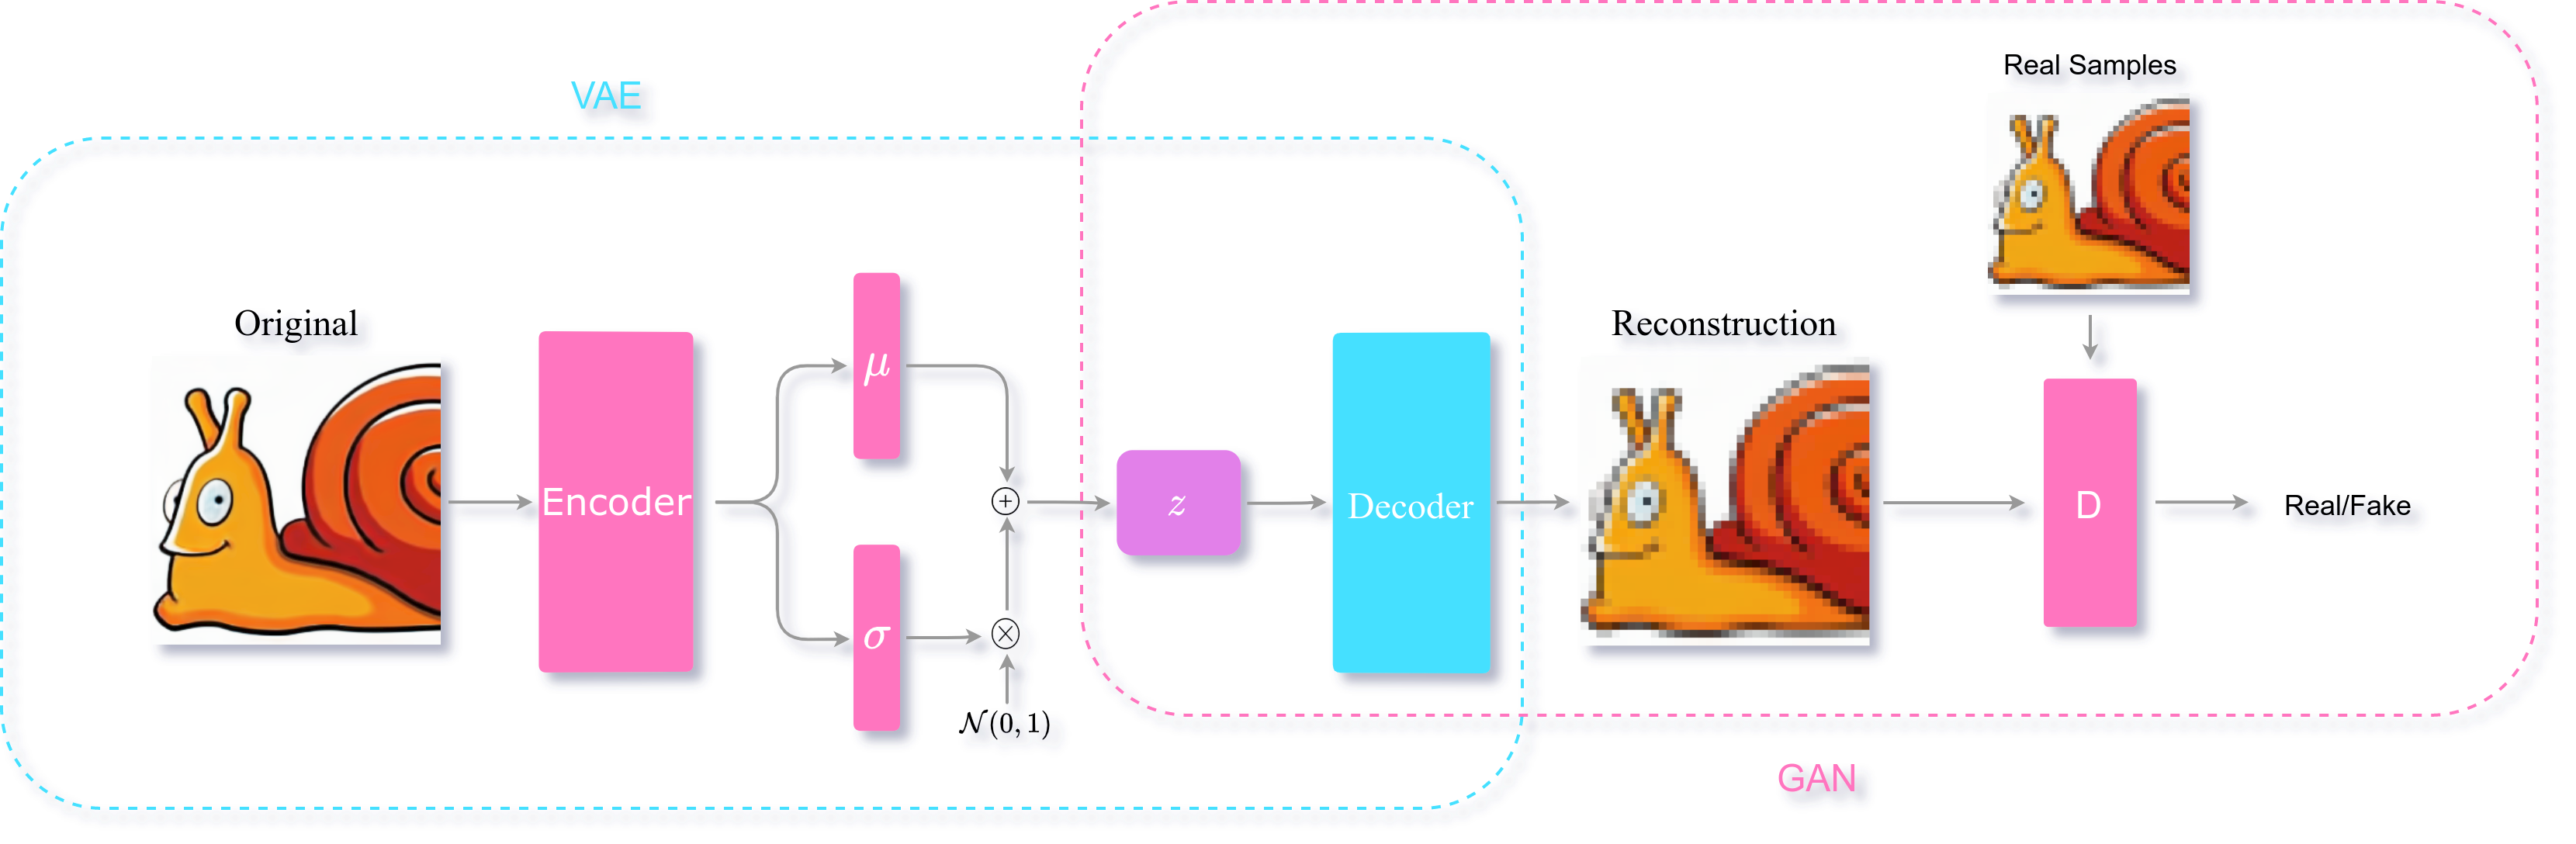
\includegraphics[scale=0.15]{figures/arch/vae_gan_arch.png}
    \caption{Illustration of the \ac{vae}-\ac{gan} architecture}
    \label{fig:vae_gan_arch}
\end{figure}

Taking the example of images again, the element-wise error is a very poor similarity metric as a small deviation in a high-level feature, like eyebrow or head rotation would lead to high error as the pixel displacement propagates through huge parts of the image. These shifts, in reality, are plausible and realistic, probably indistinguishable from the human eye. Using the discriminator as a similar metric would address this problem as the error would be low for realistic deviations of features compared to unrealistic shifts say, the noise being upside down. This can be achieved by replacing the element-wise loss of the \ac{vae} Eqn. \ref{eqn:vae_loss} with the hidden representation $D_{l}(x)$ of an intermediate layer $l$ in the discriminator that would correspond to the hidden similarity metric. The Gaussian distribution for $D_{l}(x)$ is :
    
% TODO use operator name for D, G, and functions
\begin{equation} \label{eqn:gan_similarity}
    \begin{aligned}[b]
        p\left(D_{l}(x) | z\right)=\mathcal{N}\left(D_{l}(x) | D_{l}(\tilde{x}), I\right)
    \end{aligned}
\end{equation}

Where, $\tilde{x}$ is the generated sample from the \ac{vae}'s decoder $p$. $D_{l}(tilde{x})$ is the mean of the Gaussian distribution and $I$ is the identity covariance. Replacing this as the similarity metric in \ref{eqn:vae_loss}, we get the new $\mathcal{L}_{\text {recon}}$ :

\begin{equation} \label{eqn:vaegan_recon}
    \begin{gathered}[b]
        \mathcal{L}_{\text {recon}}^{D_{l}}=-\mathbb{E}_{q(z | x)} \log p\left(D_{l}(x) | z\right)
    \end{gathered}
\end{equation}

$\mathcal{L}_{\text {recon}}^{D_{l}}$ which uses the $l^{th}$ layer of the discriminator is only the metric for the \ac{vae}, the \ac{vae}-\ac{gan} is trained on a triplet loss \ref{eqn:vaegan_loss} with $\mathcal{L}_{\text GAN}$ from Eqn. \ref{eqn:gan_loss} as a \textit{style error}. Here the generator model is the same as the decoder of the \ac{vae} as it maps from $z$ to $x$ just like $G$.

\begin{equation} \label{eqn:vaegan_loss}
    \begin{gathered}[b]
    \mathcal{L}_{\mathrm{VAEGAN}} = \mathcal{L}_{\text {recon}}^{D_{l}} +\mathcal{L}_{\text {prior }} + \mathcal{L}_{\text {GAN}}
    \end{gathered}
\end{equation}

Training \ac{vae} is hard but training \ac{gan} is harder. It is very important to consider that the training of the \ac{vae} and the \ac{gan} takes place simultaneously. While doing so it is required to \textit{limit the error propagation} of the triplet loss to the entire model. The discriminator should not learn to minimize $\mathcal{L}_{\text {recon}}^{D_{l}}$, if it does, the discriminator collapses. Better results are observed by restricting the error signal to reach the encoder $q$ as illustrated in Fig. \ref{fig:vaegan_loss_graph}. 

\begin{figure}[h]
    \centering
    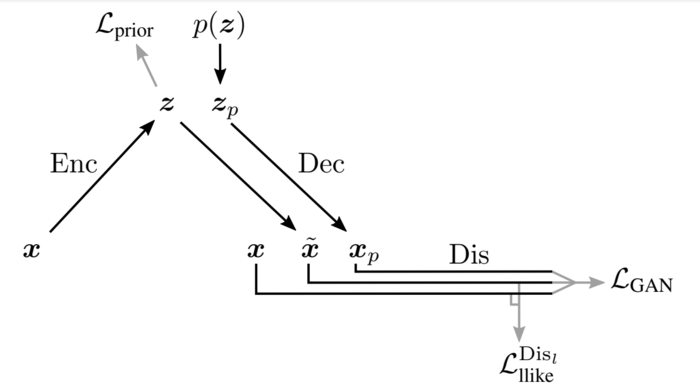
\includegraphics[scale=0.25]{figures/arch/vae_gan_loss_graph.png}
    \caption{Illustration of the data flow and the loss of \ac{vae}-\ac{gan}, where $\mathcal{L}_{\text {recon}}^{D_{l}}$ = $\mathcal{L}_{\text {llike}}^{Dis_{l}}$ \\
    Image source \cite{autoencoding_beyond_pixels}}. 
    \label{fig:vaegan_loss_graph}
\end{figure}

As discussed in \ref{subsec:bvae}, \ac{vae} as a whole has two objectives - minimize the $\mathcal{L}_{\text {recon}}$ and the $\mathcal{L}_{\text {prior}}$ and a weighing factor $\beta$ is used to maintain a trade-off between the quality of the reconstruction and the extent of disentanglement. Similarly, when it comes to \ac{vae}-\ac{gan}, the decoder alone has two objectives. One is to generate samples minimizing the $\mathcal{L}_{\text {recon}}^{D_{l}}$ and the other is to make sure that the generated samples can fool the discriminator. And the trade off is regulated by using $\gamma$ to weigh $\mathcal{L}_{\text {recon}}^{D_{l}}$ and $\mathcal{L}_{\text {\ac{gan}}}$ as in Eqn. \ref{eqn:vaegan_gamma}.
 
\begin{equation} \label{eqn:vaegan_gamma}
    \begin{gathered}[b]
        \theta_{p} \stackrel{+}{t}-\nabla_{\theta_{p}}\left(\gamma L_{\mathrm{uike}}^{D}-\mathcal{L}_{\mathrm{GAN}}\right)
    \end{gathered}
\end{equation}

In the standard \ac{gan} training, samples from the prior $p(z)$ are passed to the decoder which generates samples that are then passed to the discriminator. Interesting observation when using \ac{vae}-\ac{gan} is, sampling $x$ from the encoder $q(z|x)$ further improves the results. As the \ac{vae} tries to minimize $\mathcal{L}_{\text{prior}}$, the samples from $p(z)$ and $q(z|x)$ become similar during the training. As the generated samples $p(q(z|x))$ using the encoder are more realistic than $p(p_{prior}(z))$ using the prior, they serve as better adversarial examples for the discriminator. The $\mathcal{L}_{\mathrm{GAN}}$ loss to be used to leverage this benefit is: 

%FIXME change decoder p to be different from prior 

\begin{equation} \label{eqn:vaegan_ganloss}
    \begin{gathered}[b]
        \mathcal{L}_{\mathrm{GAN}}=\log (Dis(x))+\log (1-Dis(Dec(z)))+\log (1-Dis(Dec(Enc(x))))
    \end{gathered}
\end{equation}

%FIXME WGAN is wrong